% ==============
% Materia oscura
% ==============

Habiendo visto como el modelo estándar concuerda excelentemente con los resultados de experimentos terrestres a altas energías, veamos ahora algunas evidencias cosmológicas que apuntan a que debemos pensar en ir más allá de este modelo.

%\color{red}
%objetivo de este capítulo
%\color{black}


\section[\hspace{-0.14in}Materia oscura]{Materia oscura}

Históricamente la investigación en materia oscura comenzó en 1933 cuando el astrónomo suizo Fritz Zwicky observó que `faltaba materia' en el cúmulo de galaxias Coma \cite{zwicky}\footnote{La versión en inglés puede encontrarse aqui \cite{zwicky2009republication}.}. Posteriormente otros investigadores descubrieron que esta materia faltante, denominada \textit{materia oscura} por Zwicky, podria explicar observaciones cosmológicas como curvas de rotación planas en galaxias espirales \cite{Vera,rubin1978extended}, el efecto de lentes gravitacionales de cúmulos de galaxias y el \textit{bullet cluster} \cite{clowe2006direct}, entre otras \footnote{Las teorías de la dinámica newtoniana modificada (MOND en inglés) son alternativas a la hipótesis de la materia oscura como partícula, pero no serán discutidas en este trabajo.}. A continuación veremos brevemente cómo aparece la materia oscura en diferentes escenarios cosmológicos y porqué se piensa que su naturaleza no es de origen bariónico.


% ----------------------------
% Evidencias de materia oscura
% ----------------------------
\subsection[\hspace{-0.4in}) Evidencias]{Evidencias}




\begin{itemize}
% -----------------------------------------------------
% Evidencias de materia oscura: Cúmulos de galaxias
% -----------------------------------------------------

\item[1] \textbf{Dispersión de velocidades en cúmulos de galaxias}: En su artículo de 1933 `El corrimiento al rojo de las nebulosas extragalácticas', Fritz Zwicky estudió el cúmulo de galaxias Coma y demostró, mediante el teorema del virial, que la densidad de la materia oscura es mucho mayor que la de la materia luminosa. Suponiendo que el cúmulo de Coma es un sistema mecánicamente estacionario, el teorema del virial nos dice que la energia cinética media $\left<\mathcal{E}_k\right>$ y potencial media $\left<\mathcal{E}_p\right>$ están relacionadas por
\begin{equation}
    \left<\mathcal{E}_k\right> = - \frac{1}{2}\left<\mathcal{E}_p\right>.
    \label{virial}
\end{equation}
Para fines de estimación, supongamos una distribución uniforme de masa ($\rho$ = constante) en el cúmulo de Coma. De esta manera, si $M$ y $R$ representan su masa lumínica y radio, respectivamente, entonces su energía gravitacional $U$ es
\begin{equation}
    U=-\int_0^M G\frac{\, m(r)}{r} dm = -\frac{3}{5}\frac{GM^2}{R}.      
\end{equation}
De este resultado y la ecuación (\ref{virial}), obtenemos
\begin{equation}
    \frac{1}{2} M \left< v^2 \right> =\left<\mathcal{E}_k\right> = - \frac{1}{2}\left<\mathcal{E}_p \right> =- \frac{1}{2} U  = \frac{3}{10}\frac{GM^2}{R},
    \label{vM}
\end{equation}
lo que resulta en
\begin{equation}
    \left< v^2 \right>^{1/2} \approx \rm 80 \, km/s.
\end{equation}
Con este resultado, la dispersión de velocidades $\sigma = \left[\left< v^2 \right> - \left< v \right>^2 \right]^{1/2}\leq \left< v^2 \right>^{1/2}$ en el cúmulo de Coma está muy debajo de lo observado, \textit{i.e.} 1500 a 2000 km/s \cite{zwicky, zwicky2009republication}. Este problema hizo que Zwicky concluyera que, como $\left< v^2\right>^{1/2} \propto \sqrt{M}$ de la ecuación (\ref{vM}), el cúmulo necesitaba que su masa fuera al menos \textit{400 veces mayor} que la masa de su materia luminosa. A esta materia no observada él la llamó \textit{materia oscura}.

% -------------------------------------------------------
% Evidencias de materia oscura: Curvas de rotación planas
% -------------------------------------------------------

\item[2] \textbf{Curvas de rotación planas}: En una galaxia esférica\footnote{Hay galaxias esféricas como algunas galaxias enanas, pero hay otras que no lo son como las enanas irregulares, las galaxias elípticas y las espirales.}, de la mecánica newtoniana se espera la siguiente relación entre la velocidad de rotación $v$ y la distancia a su centro $r$,
\begin{equation}
v \propto \bigg\lbrace
\begin{array}{cc} 
r,&~\text{dentro de la galaxia} \\ 
r^{-1/2},~ &\text{fuera de la galaxia} 
\end{array}.
\label{vr-relation}
\end{equation}
Una curva de rotación es plana cuando $v$ no cae como $r^{-1/2}$ en sus afueras sino se mantiene constante. En 1970, Vera Rubin y Kent Ford mostraron la primera evidencia de curvas de rotación planas en las galaxias \cite{Vera}. En la figura \ref{rotationcurve} podemos ver la curva de rotación plana de la galaxia espiral NGC 3198.

Los modelos que intentan resolver esta discrepancia entre teoria y observación generalmente toman en consideración dos distribuciones distintas de materia. Por ejemplo, para NGC 3198 se podria usar una distribución de materia luminosa de tipo disco y un halo (esférico) de materia oscura \cite{van2004distribution}. Como resultado, los modelos de dos componentes generalmente obtienen buenos ajustes (ver Fig.\ref{rotationcurve}).

\begin{figure}[h!]
\centering
  \includegraphics[width=.8\linewidth]{Images/NGC3198.png}
  \caption[Curva de rotación de la galaxia espiral NGC 3198]{Curva de rotación de la galaxia espiral NGC 3198 \cite{van2004distribution}. La curva de rotación de la galaxia espiral NGC 3198 no puede modelarse con éxito únicamente mediante un disco de materia bariónica. Se debe agregar un halo de materia invisible para que coincida con las observaciones.}
  \label{rotationcurve}
\end{figure}


% -------------------------------------------------
% Evidencias de materia oscura: Relaciones masa-luz
% -------------------------------------------------
    
    \item[3] \textbf{Relaciones masa-luz}: La forma del universo siempre ha sido de gran interés para la humanidad. Es posible saber si es abierto, cerrado o plano determinando la relación entre su densidad de masa $\rho$ y la densidad crítica $\Omega=\rho/\rho_c$. Un universo plano $\Omega = 1$ es consistente con las observaciones \cite{Workman:2022ynf}. 
    
    Si consideramos que la masa del universo es principalmente la suma de las masas de sus partes visibles, {\it es decir} las galaxias, entonces al encontrar la relación masa-luz de una sola galaxia (suponiendo que esto sea igual para todo el universo) y multiplicarla por la luminosidad del universo debería darnos la masa del universo y, en consecuencia, $\Omega$.
    
    La luminosidad de los objetos astronómicos en el universo revela una densidad de luminosidad total de $\rho_L=2.0\pm0.7 \times 10^{8}hL_{\odot}Mpc^{-3}$ \cite{efstathiou1988analysis}. Como la densidad crítica está dada por $\rho_c=3H_0^2/8\pi G=2.775 37(13)\times 10^{11}\Omega h^2 M_{\odot}Mpc^{-3}$ \cite{patrignani2016review}, para un universo plano la relación masa-luz es \cite{peacock1999cosmological}
    \begin{equation}
    \left( \frac{M}{L} \right)_{\rm plano} = 1390h \times \left( \frac{M_\odot}{L_\odot} \right),
    \label{criticalmasstolight}
    \end{equation}
    donde $M_\odot$ y $L_\odot$ son la masa y luminosidad del sol, respectivamente, y $h=0.674$ \cite{Workman:2022ynf}.
    
   Para el cúmulo de galaxias Coma, $M/L\simeq300h$ en unidades solares \cite{zwicky,zwicky2009republication}. Dado que este valor está lejos del resultado obtenido en la ecuación (\ref{criticalmasstolight}), se necesitan más objetos masivos de baja luminosidad para obtener nuestro universo plano observado.



% ----------------------------------------------------
% Evidencias de materia oscura: Lentes gravitacionales
% ----------------------------------------------------
    \item[4] \textbf{Lentes gravitacionales}: Los cúmulos de galaxias se pueden utilizar como telescopios porque la gravedad puede `doblar' la luz. Estos cúmulos de galaxias desviarán la luz proveniente de, digamos, una sola galaxia o un grupo de ellas (ver Fig.\ref{gravlens}), y la medida de la deflexión nos dará la masa del cúmulo. Los resultados de la lente parecen coincidir con la relación masa-luz $M/L \simeq 300h$ obtenida del estudio del cúmulo de Coma \cite{zwicky,zwicky2009republication}, lo que refuerza la afirmación de que falta masa en los cúmulos de galaxias.

\begin{figure}[h]
  \centering
  \includegraphics[height=.6\linewidth]{Images/ABELL2218.png}
  \caption[Cúmulo de galaxias Abell 2218]{Cúmulo de galaxias Abell 2218 \cite{fruchterNASA}. La luz procedente de objetos luminosos situados detrás del cúmulo de galaxias Abell 2218 es desviada por éste creando arcos tenues.}
  \label{gravlens}
\end{figure}


% ------------------------------------------------------------------
% Evidencias de materia oscura: El fondo cósmico de microondas (CMB)
% ------------------------------------------------------------------
\item[5] \textbf{El fondo cósmico de microondas (CMB)}: Las mediciones de la temperatura del fondo cósmico de microondas hecho por el satétile de Planck\footnote{\textit{Planck} es la misión de la Agencia Espacial Europea para mapear el cielo midiendo la temperatura y las anisotropías de polarización de la radiación cósmica de microondas.} dio como resultado las densidades relativas $\Omega_b h^2=0.02205(28)$ para los bariones y $\Omega_{DM} h^2=0.1199(27)$ para la materia oscura fria. Ambos resultados son inferidos en el contexto del modelo cosmológico estándar $\Lambda$CDM \cite{ade2014planck} .
A partir de estos resultados, se puede ver que no sólo la materia barionica no es el componente dominante en la densidad de energía del universo, sino que además la mayor parte esta última es de composición desconocida.


\begin{figure}[h]
\centering
  \includegraphics[width=.85\linewidth]{Images/CMB.png}
\caption[Fondo cósmico de microondas]{Fondo cósmico de microondas \cite{CMBWMAP}. La imagen detallada del universo primitivo revela fluctuaciones de temperatura de 13,77 mil millones de años, que fueron las semillas que crearon las galaxias.}
  \label{CMB}
\end{figure}




% ----------------------------------------------------------------------
% Evidencias de materia oscura: La estructura a gran escala del Universo
% ----------------------------------------------------------------------
    \item[6] \textbf{La estructura a gran escala del Universo}: Como el parámetro de densidad bariónica $\Omega_b$ es muy pequeño en comparación con los otros `ingredientes' del universo, habría requerido grandes fluctuaciones en el universo primordial en la densidad bariónica para formar el número actual de galaxias observadas \cite{peacock1999cosmological}. Estas grandes fluctuaciones también significarían grandes anisotropías en el fondo cósmico de microondas. En consecuencia, la formación de galaxias en un medio puramente bariónico queda totalmente descartada por la observación de pequeñas anisotropías en el CMB (Fig.\ref{CMB}). 
    
    Por otra parte, la materia oscura fria puede formar pozos gravitacionales ideales para la formación de galaxias. Esto se debe a que ella puede desacoplarse del plasma primordial mucho antes que los bariones, lo que daria tiempo al crecimiento de inhomogeneidades y el subsecuente colapso gravitacional necesario \cite{Kolb:1990vq}. 
    
% ------------------------------------------------
% Evidencias de materia oscura: El cúmulo de balas
% ------------------------------------------------
\item[7] \textbf{El cúmulo de balas}: En los trabajos más recientes sobre cosmología observacional destacan la presencia de materia oscura en colisiones de cúmulos de galaxias. En la figura \ref{bulletcluster} vemos la colisión de dos cúmulos de galaxias fusionándose en un cúmulo doble (cúmulo de galaxias 1E 0657-56), que se conoce como {\it bullet cluster} por el gas caliente en forma de bala que se asemeja a una bala supersónica produciendo ondas de choque.

Los principales ingredientes de estas colisiones son galaxias, nubes de gas caliente y materia oscura. Como las galaxias están muy distantes unas de las otras, no participan mucho en las colisiones. Sin embargo, los gases calientes chocan, produciendo un frente de choque (Fig.\ref{bulletcluster}) y, lo más importante, separándose de la materia oscura. ¿Cómo podemos saber esto? Como se puede ver en la figura \ref{DMgravpot}, el mapa del potencial gravitacional indica claramente la presencia de dos objetos \textit{invisibles} masivos que dominan en términos de masa en este sistema y se encuentran lejos del componente lumínico dominante (el gas ionizado).



\begin{figure}[h]
\centering
  \includegraphics[width=.75\linewidth]{Images/bulletcluster.jpg}
  \caption[Cúmulo doble de galaxias 1E 0657-56: Bullet cluster]{Cúmulo doble de galaxias 1E 0657-56: el \textit{bullet cluster} \cite{clowe2006direct}. En la colisión de dos cúmulos de galaxias, el gas ionizado caliente del cúmulo más pequeño adquiere la forma de una bala, produciendo así un frente de choque en forma de arco.}
  \label{bulletcluster}
\end{figure}


\begin{figure}[h]
\centering
  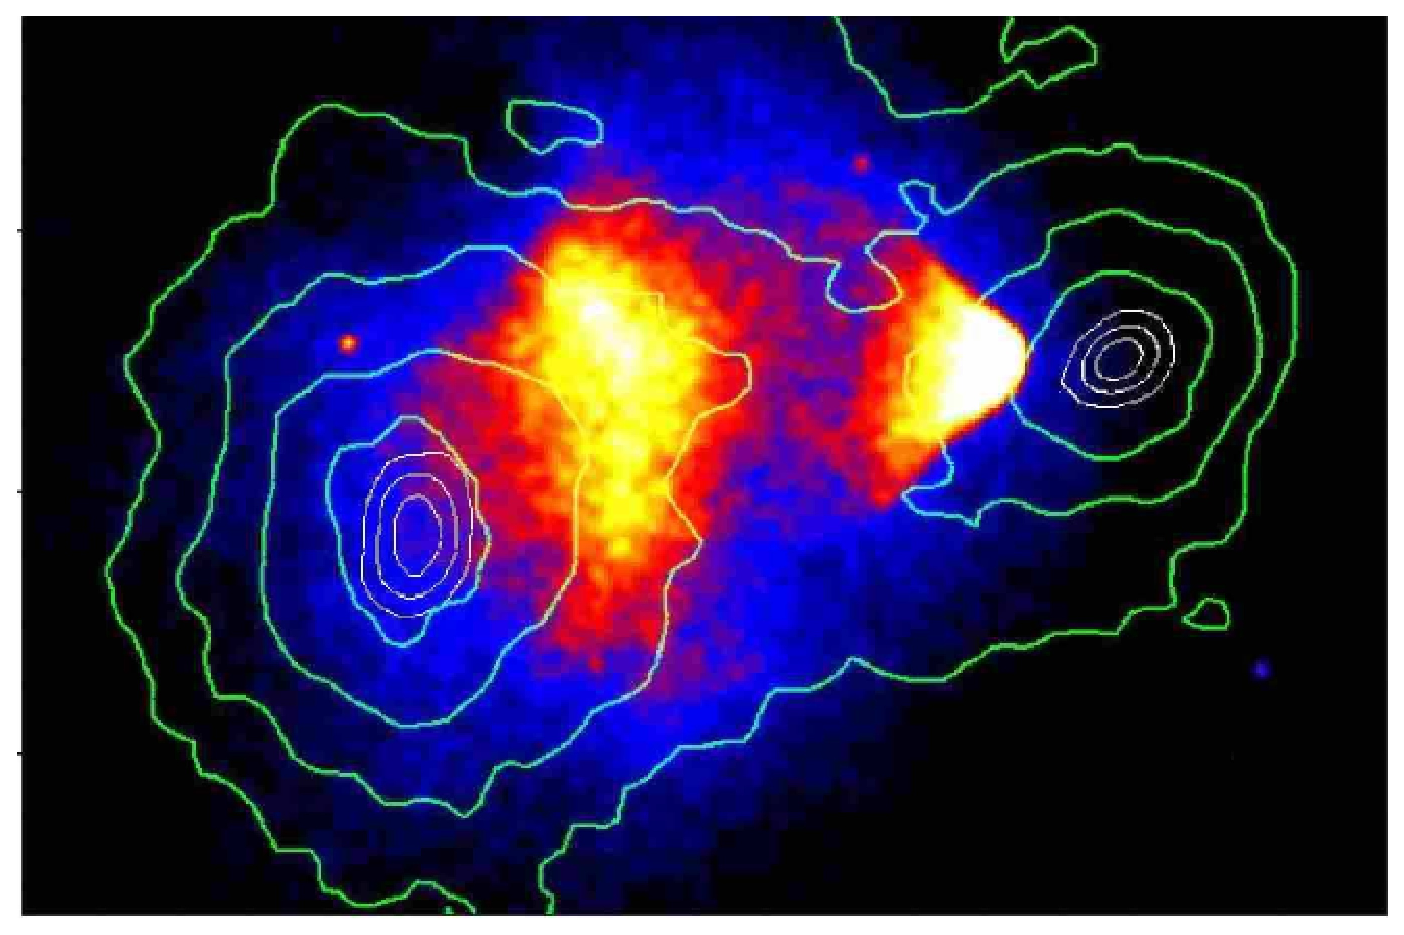
\includegraphics[width=.9\linewidth]{Images/BCgravpot.eps}
  \caption[El potencial gravitacional en el Bullet cluster]{Mapa del potencial gravitacional en la colisión de dos cúmulos de galaxias \cite{clowe2006direct}. La colisión de dos grandes cúmulos no podría exhibir esta forma de potencial gravitacional si no fuera por la materia oscura que es dominante y se ha separado del gas y las estrellas.}
  \label{DMgravpot}
\end{figure}

% -----------------------------------------
% Evidencias de materia oscura: Microlentes
% -----------------------------------------
\newpage
\item[8] \textbf{Microlentes}: Este fenómeno astronómico se basa en el efecto de lente gravitacional y utiliza el movimiento relativo entre la fuente y la lente para `aclarar' temporalmente la señal combinada. Esto significa que es posible encontrar objetos que emiten poca o ninguna luz monitoreando las curvas de luz provenientes de la fuente, las cuales son desviadas y distorsionadas.

En la figura \ref{Amplification-LigthCurve} vemos como aparecen dos picos (amplificación $A>1$) momentáneos en las bandas azul y roja en la curva de luz de una estrella en la Gran Nube de Magallanes. La curva teórica proveniente de un modelo de halo oscuro en nuestra galaxia \cite{paczynski1986gravitational} hace un fit excelente a las amplificaciones en las dos bandas \cite{alcock1993possible}. Esta no es una prueba definitiva de la presencia de materia oscura pero sí de que existe un halo oscuro masivo alrededor de la Vía Láctea.
\end{itemize}


\begin{figure}[h]
\centering
  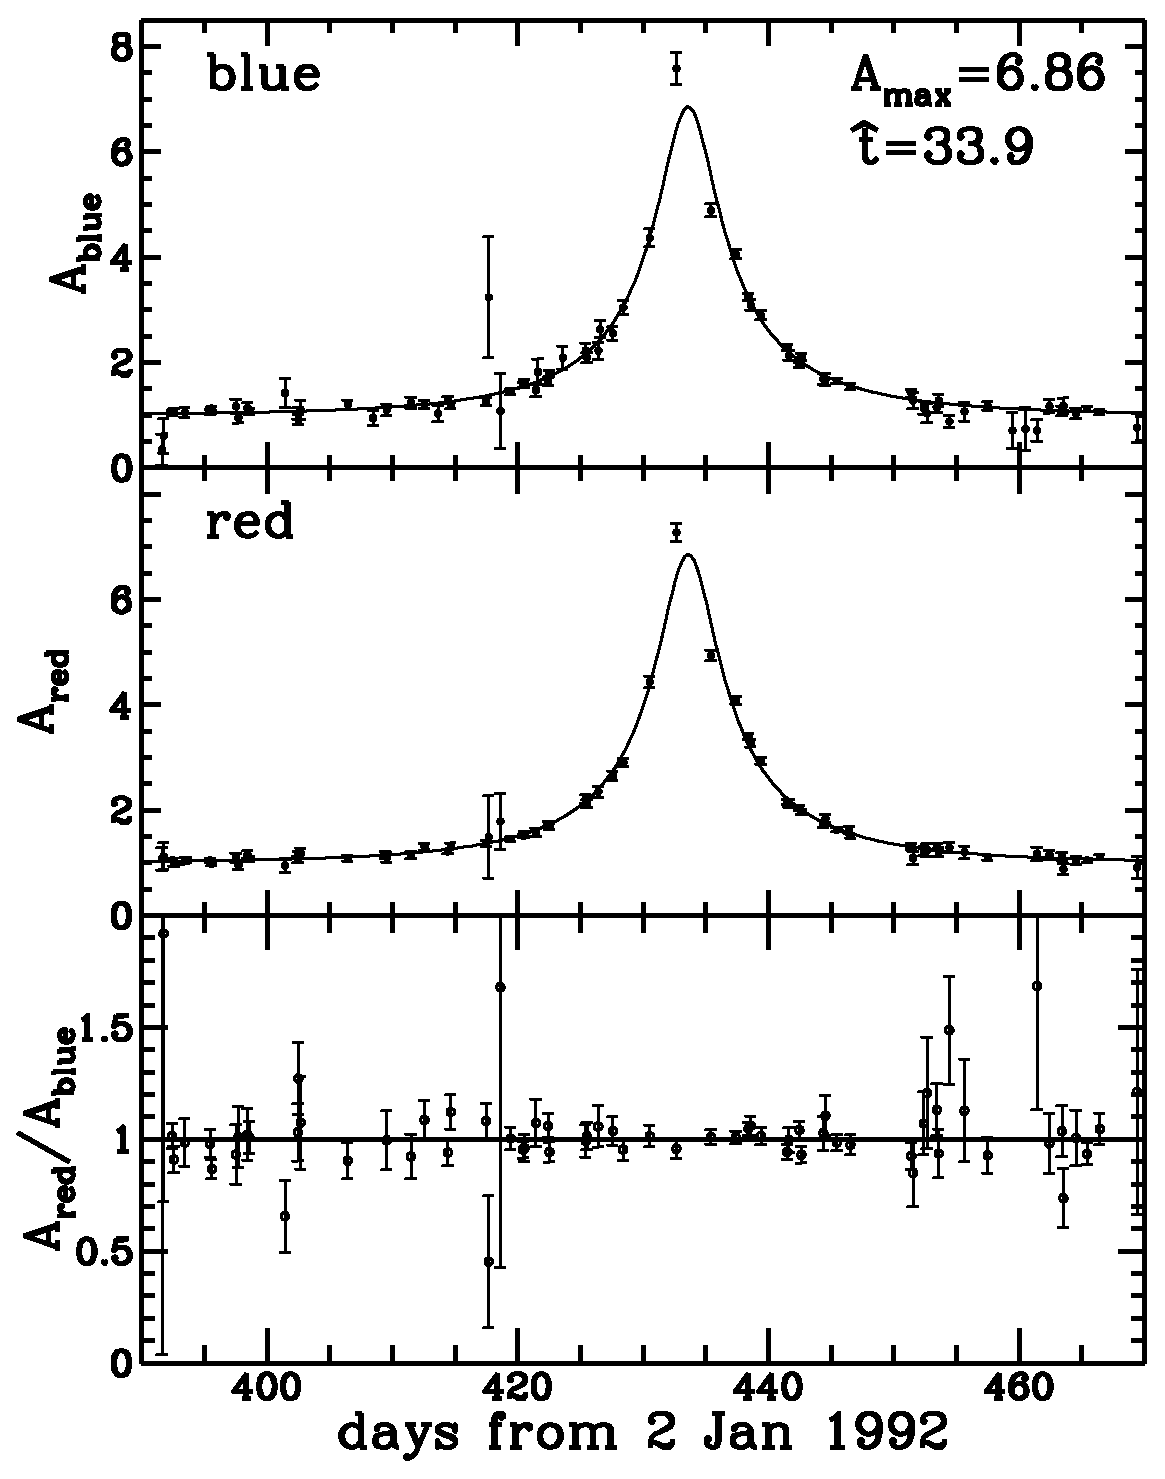
\includegraphics[height=0.8\linewidth]{Images/fluxes.eps}
  \caption[Microlentes: Curva de luz de una estrella en la nube de Magallanes]{Curva de luz de una estrella en la nube de Magallanes \cite{alcock1993possible}. La luz de fuente, en este caso una estrella, es amplificada por un objeto que no ha podido ser observado directamente. Este evento favorece la hipótesis de un halo oscuro alrededor de nuestra galaxia.}
\label{Amplification-LigthCurve}
\end{figure}



\newpage
\subsection[\hspace{-0.4in}) Partícula masiva que interactúa débilmente (WIMP)]{Partícula masiva que interactúa débilmente (WIMP)}

Como acabamos de ver, exiten fuertes evidencias de la presencia dominante, en términos cosmológicos, de (por lo menos) un tipo de materia desconocida la cual se le denomina materia oscura. A pesar de no saber con exactitud de qué está formada esta materia oscura, se puede deducir sus propiedades de manera general en el modelo cosmológico estándar \cite{Arcadi:2024ukq}. A continuación listamos  estas propiedades.

\begin{itemize}
\item[1.] \textbf{Estabilidad}. Las observaciones locales y a gran escala muestran que la materia oscura representa aproximadamente el 85$\%$ del total de materia. Como el tiempo de vida del universo es aproximadamente 13.8 Gyr, esta materia oscura debe ser estable o, caso contrário, tener un tiempo de vida média mucho mayor que la edad del universo.
\item[2.] \textbf{Interacciones débiles}. Hasta el momento no se ha observado ninguna señal de interacciones de materia oscura con la materia del modelo estándar en experimentos de detección directa como LUX, PandaX-II o XENONnT. Sumándole el hecho de que la materia oscura debe tener carga eléctrica nula para explicar, por ejemplo, las curvas de rotación de las galáxias, se puede concluir que las interacciones de la materia oscura con la materia ordinaria debe ser muy débil. 
%Experimentos de detección directa han descartado secciones de choque de WIMPs con nucleones llegando hasta $10^{-46}$ cm$^2$ (LUX y PandaX-II), $10^{-47}$ cm$^2$ XENONnT y se proyectan sentividades de hasta $10^{-49}$ cm$^2$ DARWIN.
\item[3.] \textbf{Mecanismo de producción}. Observaciones del fondo cósmico de microondas revelan que la materia oscura estaba presente en aquella época temprana del universo. Esto quiere decir que la materia oscura debe haber sido producida por algún mecanismo en el universo temprano antes de la formación del CMB, por ejemplo, freeze-out (ver apéndice). La densidad actual de materia oscura debe ser explicada por este mecanismo.
\item[4.] \textbf{Adecuado para la formación de estructuras}. La materia oscura es uno de los principales actores en la formación de galaxias ya que provee el pozo de potencial para capturar la materia ordinaria. Para que esto suceda, la materia oscura debe ser no relativista y muy abundante en la época de igualdad materia-radiación. 
\item[5.] \textbf{Autointeracciones}. Como vimos en el item 2, las interacciones de la materia oscura con la materia ordiaria debe ser muy débil. Sin embargo, esto no descarta la posibilidad de que la materia oscura pueda interactuar consigo misma o con partículas de un sector oscuro. En particular, para explicar las observaciones del cúmulo de balas (bullet cluster) se debe tener $\sigma/m <$ 1 cm$^2$/g \cite{Markevitch:2003at}.
\end{itemize}

Una clase popular de candidatos a materia oscura son partículas masivas que interactúan débilmente (WIMP)\footnote{Weakly Interactive Massive Particle.}. Estas partículas generalmente tienen una sección de choque `correcta' $\left< \sigma v\right> \sim 3 \times 10^{-26}$ cm$^3$/s para masas de GeV$-$TeV, lo que las hace fuertes candidatos \cite{profumo2017introduction}. Los WIMPs obtienen su densidad de relíquia del proceso de desacoplamiento del plasma primordial en las primeras etapas de la historia del universo lo que les da una densidad comóvil constante la cual se mantiene hasta el presente.

% --------------------------------------------------------------------------------------------------------
\section[\hspace{-0.14in}Detección directa e indirecta de materia oscura]{Detección directa e indirecta de materia oscura}
% -------------------------------------------------------------------------------------------------------- 

La búsqueda de materia oscura se da a través de experimentos de detección directa, detección indirecta y producción en colosionadores. Si bien la materia oscura interactua muy poco con las partículas del modelo estándar, procesos a nivel de loop podrían dar señales de ella. En la figura \ref{fig_DMsearches} se muestra como estos procesos provenientes de nueva física podrían producir partículas de materia oscura en experimentos con colisionadores como el LHC y como puede darse la detección directa e indirecta de materia oscura. Si bien estas búsquedas son complementarias, cada una de ellas es un tema muy amplio y por eso dejaremos este estudio para futuros trabajos. Sin embargo, comentaremos un poco sobre estas búsquedas de materia oscura.

%en esta tesis nos enfocaremos en poner límites a un candidato a materia oscura proveniente del $3-3-1$ Económico por medio de detección indirecta. %ya que detección directa tiene el background irreducible de neutrinos (ver Strumia's review) Queiroz:2016awc

\begin{figure}[h]
\centering
\includegraphics[scale=0.45]{Images/DM-searches.pdf}
\caption[Interacciones de la materia oscura]{Diferentes tipos de interacción de la materia oscura ($\chi$) con partículas del modelo estándar (ME). Nótese que los procesos horizontales determinan la densidad de materia oscura proveniente del freeze-out térmico ya que este proceso cambia el número de partículas de materia oscura.}
\label{fig_DMsearches}
\end{figure}


\subsection[\hspace{-0.4in}) Detección directa]{Detección directa}
La detección directa de materia oscura es un enfoque experimental que busca identificar interacciones entre partículas de materia oscura y materia ordinaria. Este tipo de detección se basa en la hipótesis de que las partículas de materia oscura, como los WIMPs, podrían interactuar débilmente con núcleos atómicos a través de colisiones elásticas, causando un retroceso nuclear detectable. Para ello, los experimentos utilizan detectores extremadamente sensibles, ubicados en laboratorios subterráneos para minimizar el ruido de fondo proveniente de rayos cósmicos y otras fuentes de radiación \cite{profumo2017introduction}. 

Los detectores suelen emplear tecnologías avanzadas, como cristales de germanio, xenón líquido o argón líquido, que pueden registrar pequeñas cantidades de energía liberadas en los retrocesos nucleares. La señal de materia oscura esperada es extremadamente débil\footnote{La energía depositada por las partículas de materia oscura en los detectores es del orden de eV$-$keV \cite{Cirelli:2024ssz}.} , por lo que estos experimentos están diseñados para discriminar entre posibles eventos de materia oscura y señales de fondo, como radiación gamma o neutrones. Además, las técnicas de análisis buscan patrones característicos, como una modulación anual debida al movimiento relativo de la Tierra a través del halo de materia oscura.

\begin{figure}[h]
\centering
\includegraphics[scale=0.55]{Images/WIMP-DD.pdf}
\caption[\hspace{0.05in}Límites en la sección de choque de los WIMPs]{Límites en la sección de choque (independiente del spin) de un WIMP con nucleones \cite{Cooley:2014aya}.}
\label{WIMPDD}
\end{figure}

Aunque hasta ahora no se ha detectado directamente materia oscura, estos experimentos han impuesto límites estrictos sobre la probabilidad de interacción (sección de choque) y en función de las masas de las partículas candidatas a materia oscura, ver figura \ref{WIMPDD}. 

\subsection[\hspace{-0.4in}) Perfiles de materia oscura]{Perfiles de materia oscura}
%\subsection{Fermi-LAT}
La materia oscura en las galáxias se encuentra distribuida en toda su extensión y por este motivo estas se modelan típicamente usando un halo de materia oscura. La forma de este halo depende del tipo de galáxia. Perfiles comúnmente usados en la literatura son Navarro-Frenk-White (NFW) \cite{Navarro:1995iw} y Einasto \cite{einasto1965kinematics}, los cuales provienen de simulaciones de N-cuerpos de alta resolución, ver figura \ref{profiles}.

\begin{figure}[h]
\centering
\includegraphics[scale=0.5]{Images/profiles.pdf}
\caption[\hspace{0.1in}Perfiles de densidad de materia oscura]{Perfiles de densidad de materia oscura: NFW, Einasto y NFW cored (NFWc) \cite{Angel:2023rdd}.}
\label{profiles}
\end{figure}

NFW es el perfil de materia oscura más popular ya que se basa en materia oscura fria que `no colisiona'\footnote{Collisionless cold dark matter.}, esto es interacciones puramente gravitacionales. Este perfil consigue reproducir bien las curvas de rotación de varias galáxias, sin embargo, en el centro de ellas aparece un problema: la densidad central de NFW es mayor de la requerida para explicar la parte central de las curvas de rotación de las galáxias. Ante esto, otras opciones aparecen, tales como NFWc\footnote{Contracted NFW.} y Einasto. La primera viene de generalizar NFW usando
\begin{equation}
\rho (r) = \frac{\rho_0}{(r/r_s)^\gamma (1+r/r_s)^{3-\gamma}},
\end{equation}
donde $\gamma$ es un parámetro libre: $\gamma =1$  para NFW y $\gamma = 1.3$ para NFWc. Para Einasto tenemos
\begin{equation}
\rho (r) = \rho_0 \exp \left\{ - \frac{2}{\alpha} \left[ \left( \frac{r}{r_0}\right)^\alpha -1 \right] \right\}.
\end{equation} 

\subsection[\hspace{-0.4in}) Detección indirecta]{Detección indirecta}
La materia oscura, a pesar de ser estable en escalas cosmológicas, podría dar señales de su presencia al aniquilarse en regiones de alta concentración como el centro galáctico o galáxias enanas y producir partículas del modelo estándar que podamos detectar en la Tierra. El programa de detección indirecta de materia oscura se basa en identificar fotones, neutrinos y rayos cósmicos provenientes de estas aniquilaciones\footnote{También se buscan los productos de decaimientos de materia oscura, pero no abordaremos ese tema en este trabajo.}. Los fotones y los neutrinos son de particular interés porque viajan en línea recta (a diferencia de los rayos cósmicos que son cargados eléctricamente) y por eso se puede saber de dónde vienen. Los neutrinos, a pesar de ser muy numerosos, son difíciles de detectar ya que estos tienen secciones de choque muy pequeñas. Por otro lado, los fotones tienen secciones de choque mayores y pueden ser producidos con un espectro de energía contínuo o discreto (línea) proveniente de aniquilaciones de materia oscura ($\mathcal{DM}\, \mathcal{DM} \to \gamma \gamma$) donde la energía de los fotones es $E_\gamma = m_\mathcal{DM}$. En la figura \ref{fig:g_Servant} se muestra como ejemplo el flujo de fotones para una materia oscura de 300 GeV \cite{Jackson:2013pjq}.
\begin{figure}[h]
\centering
\includegraphics[scale=1]{Images/fig_Servant.pdf}
\caption[Espectro de rayos gamma (línea)]{Espectro de rayos gamma para un modelo donde la materia oscura tiene 300 GeV de masa. El pico que se distingue del espectro contínuo viene de la producción directa $\mathcal{DM}\, \mathcal{DM} \to \gamma \gamma$ donde $E_\gamma = m_\mathcal{DM} =300$ GeV. Imagen adaptada de \cite{Jackson:2013pjq}.}
\label{fig:g_Servant}
\end{figure}

La forma de calcular este flujo de fotones\footnote{Flujo diferencial de una dirección angular $d\Omega$.} llegando a la Tierra es (vea, por ejemplo, \cite{Cirelli:2010xx,Queiroz:2016awc,Slatyer:2021qgc})
\begin{equation}
\frac{d\Phi_{\gamma}}{d\Omega \, dE} = \frac{1}{2} \frac{r_\odot}{4\pi} \left( \frac{\rho_\odot}{m_\mathcal{DM}} \right)^2 J \sum_f \left< \sigma \, v \right>_f \frac{dN_\gamma^f}{dE},
\end{equation}
donde $r_\odot=8.33$ kpc es la posición del sol respecto al centro galáctico, $\rho_\odot=0.3$ GeV/cm$^3$ es la densidad de la materia oscura cerca al sol \cite{gillessen2009monitoring}, $m_\mathcal{DM}$ es la masa de la materia oscura, $dN_\gamma^f/dE$ es el espectro de energia de los fotones producidos por aquinilación, el factor $J$ está dado por
\begin{equation}
J = \int_{\rm l.o.s.} \frac{ds}{r_\odot} \left( \frac{\rho (r(s,\theta))}{\rho_\odot} \right)^2,
\end{equation}
y $\left< \sigma \, v \right>_f$ es la sección de choque térmicamente promediada en el canal con estado final $f$. Esta ecuación es válida para partículas de materia oscura que sean auto-conjugadas, por ejemplo fermiones de Majorana. Cuando este no sea el caso, debe promediarse sobre partículas y antipartículas, entonces aparece un factor multiplicativo extra, $1/2$.




%\subsection{H.E.S.S.}

%El Sistema Estereoscópico de Alta Energía\footnote{High Energy Stereoscopic System.} (H.E.S.S.) es un arreglo de telescópios atmosféricos Cherenkov para la investigación de los rayos gamma cósmicos en el rango de energía de los fotones de GeV$-$TeV.

%Estos rayos gamma podrían provenir de la aniquilación de materia oscura en regiones altamente densas como el centro de la galáxia. Se espera que de las aniquilaciones de materia oscura en quarks, leptones pesados o bosones vectoriales, junto con una emisión secundaria proveniente de scattering de Compton inverso asi como de bremsstrahlung de electrones producidos en la cadena de decaimientos, produzca un contínuo de rayos gamma. El background de fotones provenientes de otros procesos astrofísicos hace que la distinción de esta señal algo no trivial \cite{HESS:2018cbt}.

%Por ortra parte, los decaimientos en líneas de rayos gamma\footnote{$\gamma-ray$ lines.} provenientes de la aniquilación de materia oscura en `reposo' ($v \sim 10^{-3}c$) en $\gamma+X$ donde $X=\gamma, Z, h$ u otras partículas del sector oscuro, producen una línea espectral angosta con energía $E_\gamma =m_{\rm DM}(1-m_X^2/4m^2_{\rm DM})$, la cual está limitada por la resolución del detector. Para H.E.S.S. la resolución de energía es $10\%$. Cuando la materia oscura se aniquila en partículas cargadas, existen rayos gamma adicionales provenientes de radiación en estado final\footnote{Final state radiation (FSR).} y bremsstrahlung interno.

%Como vimos anteriormente, la distribución de materia oscura en la galáxia es muy importante para el cálculo del flujo de rayos gamma. La colaboración H.E.S.S. trabajó con dos perfiles: NFW y Einasto. Los resultados de 10 años de observaciones de H.E.S.S. se muestran en la figura \ref{HESS_sigmav}. Se puede ver que llegan a poner límites superiores a $\left< \sigma \, v \right>$ hasta $10^{-27}$cm$^3$/s para el perfil NFW y aún menores abajo para Einasto. Como comparación se muestran también resultados de otras colaboraciones como la de Fermi-LAT que es dominante en una región donde no llega H.E.S.S.


\begin{figure}[h!]
\centering
\includegraphics[scale=0.5]{Images/HESS.pdf}
\caption[Limites para $\left< \sigma \, v \right>$ provenientes de H.E.S.S.]{Limite superior para $\left< \sigma \, v \right>$ para el proceso de aniquilación de materia oscura en rayos gammas proveniente de 10 años de observaciones del halo galáctico interno. Imagen adaptada  de \cite{HESS:2018cbt}.}
\label{HESS_sigmav}
\end{figure}

\newpage
% ----------------------------------------------------------------------------------- 
\section[\hspace{-0.14in}Modelo $\nu_R$-331]{Modelo $\nu_R$-331}
% -----------------------------------------------------------------------------------

%\color{red}
%Leer paper de Vicente: resumen 3-3-1
%\color{black}

Los modelos $3-3-1$ surgen al reemplazar el grupo de gauge del modelo estándar G$_{\rm SM} \equiv SU(3)_C \times SU(2)_L \times U(1)_Y$ por G$_{\rm 3-3-1} \equiv SU(3)_C \times SU(3)_L \times U(1)_X$, donde $C$ y $L$ son color y quiralidad izquierda, respectivamente, y $X$ representa una nueva carga diferente de la hipercarga $Y$ del modelo estándar.

Aqui, el operador de carga eléctrica se puede escribir como \cite{Pleitez:2021abk},
\begin{equation}
Q_{\beta}(X) = a T_3 + \beta T_8 + X \mathds{1}_{3\times 3},
\end{equation}
donde $T_3$ y $T_8$ son las matrices diagonales de Gell-Mann, y $\mathds{1}_{3\times 3}$ es la matriz identidad. 

Para fines prácticos, en este trabajo seguiremos \cite{sanchez2019vacuum} tomando\footnote{Otros valores para $\beta$ son $\sqrt{3},-\sqrt{3}$ y $1/\sqrt{3}$.} $a=1$, $\beta = -1/\sqrt{3}$ y trabajando con el sector escalar más simple para modelos sin cargas eléctricas exóticas \cite{Foot:1994ym,Ponce:2001jn}. A este modelo se le conoce en la literatura como modelo $\nu_R-331$ \cite{Singer:1980sw}.

En este modelo, por ejemplo, los neutrinos de mano derecha $N_a \ (a=1,2,3)$ se encuentran juntos con los leptones del modelo estándar en el mismo multiplete de $SU(3)_L$,
\begin{eqnarray}
\text{Leptones} : \text{L}_{aL} = \left( \begin{array}{c}
\nu_a \\ \ell_a  \\ N_a^c
\end{array} \right)_L &\sim & (1, \textbf{3},-1/3), \nonumber \\
\ell_{aR} &\sim & (1,1,-1),
\end{eqnarray}
mientras que en el sector de quarks aparecen nuevos quarks `tipo up' y `tipo down',
\begin{eqnarray}
\text{Quarks} : \text{Q}_{L} = \left( \begin{array}{c}
u_1 \\ d_1  \\ u_4
\end{array} \right)_L &\sim &  (\textbf{3}, \textbf{3},1/3), \
\text{Q}_{bL} = \left( \begin{array}{c}
d_b \\ u_b  \\ d_{b+2}
\end{array} \right)_L \sim  (\textbf{3}, \bar{\textbf{3}},0), \nonumber \\
u_{sR} &\sim & (3,1,2/3), \hspace{1.15in} d_{tR} \sim  (3,1,-1/3), \nonumber \\
\end{eqnarray}
donde $b=2,3$, $s=1,...,4$ y $t=1,...,5$. Nótese que hay cuatro quarks tipo up y cinco tipo down ya que están organizados en tres tripletes y por eso el número total de quarks es nueve.

En el sector escalar mínimo tenemos tres tripletes escalares que se transforman bajo el grupo de gauge G$_{\rm 3-3-1}$ de esta manera,
\begin{eqnarray}
\rho &=& \left( \begin{array}{c}
\rho_1^+ \\ \rho_2^0  \\ \rho_3^+
\end{array} \right)  \sim (1, \textbf{3}, \ 2/3)
\end{eqnarray}

\begin{eqnarray}
\eta &=& \left( \begin{array}{c}
\eta_1^0 \\ \eta_2^-  \\ \eta_3^0
\end{array} \right) \sim (1, \textbf{3}, -1/3)
\end{eqnarray}


\begin{eqnarray}
\chi &=& \left( \begin{array}{c}
\chi_1^0 \\ \chi_2^-  \\ \chi_3^0
\end{array} \right) \sim (1, \textbf{3}, -1/3)
\end{eqnarray}

Para el $\nu_R-331$, usualmente se asume una simetría $\mathbb{Z}_2$ donde todos los campos son pares bajo esta simetría con excepción del triplete escalar $\chi$, un quark tipo up y dos quarks tipo down,
\begin{equation}
\mathbb{Z}_2^{3-3-1} : \chi \to - \chi, \ u_{4R} \to - u_{4R}, \ d_{4R} \to - d_{4R}, \ d_{5R} \to - d_{5R}.
\end{equation}
Esta simetría es motivada por la fenomenología ya que mitiga problemas de corrientes neutras que cambian de sabor\footnote{Flavor changing neutral currents (FCNC).} \cite{GomezDumm:1993oxo} y permite la implementación del mecanismo de Peccei-Quinn \cite{Montero:2011tg}.


De esta manera, en el potencial escalar tendremos términos invariantes por $\mathbb{Z}_2$ y otros que no lo son,
\begin{equation}
V^{3-3-1} = V_{\mathbb{Z}_2} + V_{\slashed{\mathbb{Z}}_2}.
\end{equation}
Los términos invariantes por $\mathbb{Z}_2$ son de dimensión de masa 2 y 4,
\begin{equation}
V_{\mathbb{Z}_2} = V_{\mathbb{Z}_2}^{(2)} + V_{\mathbb{Z}_2}^{(4)},
\end{equation}
\begin{eqnarray}
V_{\mathbb{Z}_2}^{(2)} &=& -\mu_\rho^2 \left( \rho^{\dagger}\rho \right) -\mu_\eta^2 \left( \eta^{\dagger}\eta \right) -\mu_\chi^2 \left( \chi^{\dagger}\chi \right), \nonumber \\
V_{\mathbb{Z}_2}^{(4)} &=& \lambda_1 \left( \rho^{\dagger}\rho \right)^2 + \lambda_2 \left( \eta^{\dagger}\eta \right)^2 + \lambda_3 \left( \chi^{\dagger}\chi \right)^2 \nonumber \\
&+& \lambda_4 \left( \rho^{\dagger}\rho \right) \left( \chi^{\dagger}\chi \right) + \lambda_5 \left( \eta^{\dagger}\eta \right) \left( \chi^{\dagger}\chi \right) + \lambda_6 \left( \rho^{\dagger}\rho \right) \left( \eta^{\dagger}\eta \right) \nonumber \\
&+& \lambda_7 \left( \rho^{\dagger}\chi \right) \left( \chi^{\dagger}\rho \right) + \lambda_8 \left( \eta^{\dagger}\chi \right) \left( \chi^{\dagger}\eta \right) + \lambda_9 \left( \rho^{\dagger}\eta \right) \left( \eta^{\dagger}\rho \right) \nonumber \\
&+& \lambda_{10} \left( \eta^{\dagger}\chi \right)^2 + \text{H.c.},
\end{eqnarray}
mientras que los que no respetan $\mathbb{Z}_2$, son de dimensión 2, 3 y 4,
\begin{equation}
V_{\slashed{\mathbb{Z}}_2} = V_{\slashed{\mathbb{Z}}_2}^{(2)} + V_{\slashed{\mathbb{Z}}_2}^{(3)} + V_{\slashed{\mathbb{Z}}_2}^{(4)}.
\end{equation}
Los términos de dimensión de masa 2 y 3 son términos de ruptura suave\footnote{Soft-breaking term. Una simetría global se rompe suavemente cuando los términos de dimensión de masa 4 del lagrangiano son invariantes por esta simetría, pero los de dimensión 2 ó 3 no lo son. La introducción de términos de ruptura suave en el modelo no estropea su renormalizabilidad (vea \cite{Ferreira:2022gjh}).} y por eso los agrupamos en $V_{soft}$,
\begin{eqnarray}
V_{\slashed{\mathbb{Z}}_2}^{(4)} &=& \lambda_{11}\left( \chi^{\dagger}\eta \right) \left( \eta^{\dagger}\eta \right) + \lambda_{12}\left( \chi^{\dagger}\eta \right) \left( \chi^{\dagger}\chi \right)   \nonumber \\
&+& \lambda_{13}\left( \chi^{\dagger}\eta \right) \left( \rho^{\dagger}\rho \right) + \lambda_{14}\left( \chi^{\dagger}\rho \right) \left( \rho^{\dagger}\eta \right) + \text{H.c}, \nonumber \\
V_{soft} &=& - \mu_{\eta\chi}^2 \left( \eta^{\dagger} \chi \right) + \frac{f \,}{\sqrt{2}} \varepsilon_{ijk} \rho_i \eta_j \chi_k + \text{H.c}.
\end{eqnarray}

De esta manera, el potencial escalar formado por los términos invariantes por $\mathbb{Z}_2$ y los términos de ruptura suave es, 
\begin{eqnarray}
V^{3-3-1} &=& -\mu_\rho^2 \left( \rho^{\dagger}\rho \right) -\mu_\eta^2 \left( \eta^{\dagger}\eta \right) -\mu_\chi^2 \left( \chi^{\dagger}\chi \right) - \mu_{\eta\chi}^2 \left( \eta^{\dagger} \chi \right)\nonumber \\
&+& \lambda_1 \left( \rho^{\dagger}\rho \right)^2 + \lambda_2 \left( \eta^{\dagger}\eta \right)^2 + \lambda_3 \left( \chi^{\dagger}\chi \right)^2 \nonumber \\
&+& \lambda_4 \left( \rho^{\dagger}\rho \right) \left( \chi^{\dagger}\chi \right) + \lambda_5 \left( \eta^{\dagger}\eta \right) \left( \chi^{\dagger}\chi \right) + \lambda_6 \left( \rho^{\dagger}\rho \right) \left( \eta^{\dagger}\eta \right) \nonumber \\
&+& \lambda_7 \left( \rho^{\dagger}\chi \right) \left( \chi^{\dagger}\rho \right) + \lambda_8 \left( \eta^{\dagger}\chi \right) \left( \chi^{\dagger}\eta \right) + \lambda_9 \left( \rho^{\dagger}\eta \right) \left( \eta^{\dagger}\rho \right) \nonumber \\
&+& \lambda_{10} \left( \eta^{\dagger}\chi \right)^2 + \frac{f \,}{\sqrt{2}} \varepsilon_{ijk} \rho_i \eta_j \chi_k + \text{H.c}.
\label{preV331Ec}
\end{eqnarray}
En \cite{sanchez2019vacuum} se muestra como la redefinición de los campos escalares dada por $\rho_i\to e^{-i\delta_{15}} \rho_i,\eta_i\to e^{-i\delta_{10}/4} \eta_i, \chi_i\to e^{i\delta_{10}/4} \chi_i$ donde $\lambda_{10} = |\lambda_{10}|e^{i\delta_{10}}$ y $f \, = |f| \,e^{i\delta_{15}}$ deja el potencial invariante con excepción del término proporcional a $\mu_{\eta \chi}^2$. Sin embargo, más adelante se verá que este parámetro es nulo al resolver las ecuaciones $tadpole$. Sabiendo esto, por simplicidad, asumiremos que todas los parámetros son reales y trabajaremos con el siguiente potencial escalar\footnote{Nótese que en \cite{sanchez2019vacuum} el orden de los campos $\eta$ y $\rho$ en el término de soft-breaking está invertido y por eso lleva un signo negativo.} al que llamaremos potencial del $\nu_R-331$,
\begin{eqnarray}
V^{3-3-1} &=& -\mu_\rho^2 \left( \rho^{\dagger}\rho \right) -\mu_\eta^2 \left( \eta^{\dagger}\eta \right) -\mu_\chi^2 \left( \chi^{\dagger}\chi \right) \nonumber \\
&+& \lambda_1 \left( \rho^{\dagger}\rho \right)^2 + \lambda_2 \left( \eta^{\dagger}\eta \right)^2 + \lambda_3 \left( \chi^{\dagger}\chi \right)^2 \nonumber \\
&+& \lambda_4 \left( \rho^{\dagger}\rho \right) \left( \chi^{\dagger}\chi \right) + \lambda_5 \left( \eta^{\dagger}\eta \right) \left( \chi^{\dagger}\chi \right) + \lambda_6 \left( \rho^{\dagger}\rho \right) \left( \eta^{\dagger}\eta \right) \nonumber \\
&+& \lambda_7 \left( \rho^{\dagger}\chi \right) \left( \chi^{\dagger}\rho \right) + \lambda_8 \left( \eta^{\dagger}\chi \right) \left( \chi^{\dagger}\eta \right) + \lambda_9 \left( \rho^{\dagger}\eta \right) \left( \eta^{\dagger}\rho \right) \nonumber \\
&+& |\lambda_{10}| \left( \eta^{\dagger}\chi \right)^2 + \frac{|f| \,}{\sqrt{2}} \varepsilon_{ijk} \rho_i \eta_j \chi_k + \text{H.c},
\label{V331Ec}
\end{eqnarray} 
Nótese que H.c. solo se aplica a los dos últimos términos. Como $|\lambda_{10}|\geq 0$ y $|f|>0$, a partir de ahora omitiremos el símbolo de valor absoluto por motivos de notación y simplemente asumiremos $\lambda_{10}$ como no negativo y $f$ como positivo.

En los modelos $3-3-1$ es usual asumir que el rompimiento espontáneo de simetria\footnote{Spontaneous symmetry breaking (SSB).} se da en dos pasos,
\begin{equation}
SU(3)_L\times U(1)_X \xrightarrow[]{  v_\chi  } SU(2)_L\times U(1)_Y \xrightarrow[]{ v_{\rm SM} = \sqrt{v_\rho^2+ v_\eta^2} } U(1)_{\rm em} ,
\end{equation}
donde $v_{\rm SM} \simeq 246$ GeV y los VEVs de los tripletes escalares son,
\begin{equation}
\langle \rho \rangle =  \frac{1}{\sqrt{2}} \left( 
\begin{array}{c}
0 \\ v_\rho \\ 0 
\end{array}
\right), \
\langle \eta \rangle =  \frac{1}{\sqrt{2}} \left( 
\begin{array}{c}
v_\eta \\ 0 \\ 0 
\end{array}
\right), \
\langle \chi \rangle =  \frac{1}{\sqrt{2}} \left( 
\begin{array}{c}
0 \\ 0 \\ v_\chi
\end{array}
\right).  
\end{equation}

En principio, $\eta_3^0$ y $\chi_1^0$ también podrian obtener un VEV, pero en este caso bosones de Nambu-Goldstone (NG) aparecen en el espectro de la teoría \cite{sanchez2018new}. 

%Los NG que son comidos por los bosones vectoriales son
%\begin{equation}
%\left\{ \chi_2^{\pm}, s_\beta \, \eta_2^{\pm} - c_\beta \, \rho_1^{\pm}, \text{Im} (\chi_3^0), s_\beta \text{Im} (\eta_1^0) - c_\beta \text{Im} (\rho_2^0) , \text{Im} (\chi_1^0), -\text{Re} (\chi_1^0)  \right\}. 
%\end{equation}  

Después del rompimiento espontáneo de simetria, aparecen nuevas partículas. Algunas de ellas son muy pesadas ya que sus masas son proporcionales a la escala de energía de los $3-3-1$ y otras poseen masas que podrian estar cercanas a la masa del bosón de Higgs. Calculamos estas masas para los escalares y bosones vectoriales, y las mostramos en la tabla \ref{masses331}. Allí hemos usado las siguientes definiciones provenientes de \cite{Okada:2016whh},
\begin{equation}
\tan \beta \equiv \frac{v_{\eta}}{v_\rho}, \hspace{0.25in} \tan \theta_{331} \equiv \frac{2g_X}{\sqrt{3}g}, \hspace{0.25in} c_W \equiv \frac{1}{2} \sqrt{1+3c_{331}^2},
\end{equation}
donde $c_W = \cos \theta_W$, $\theta_W$ es el ángulo de Weinberg. La primera y segunda definición son dadas por conveniencia, mientras que la tercera hace que la masa del bosón $Z$ concuerde con la del modelo estándar en el límite $v_\chi \to \infty$, \textit{i.e.} $m_Z = g\, v_{\rm SM}/2c_W$.


En varios trabajos se muestran que la escala de energía de los $3-3-1$ debe ser mayor a (por lo menos) 10 TeV \cite{Salazar:2015gxa,Queiroz:2016gif,Alvarez-Salazar:2019cxw}. Por otro lado, la escala de soft-breaking $f$ que aparece en el término trilinear del potencial escalar ha sido poco estudiada y su valor no está muy restringido, pudiendo este ser mucho menor a la escala electrodébil $f \ll v_{\rm SM}$, del orden de la escala electrodébil $f \sim \mathcal{O} (v_{\rm SM})$, del orden de la escala de energía de los $3-3-1$ $f \sim \mathcal{O} (v_{\chi})$ o mayor a todas las otras escalas de energía $f \gg v_\chi$ \cite{Pinheiro:2022bcs}.

En este trabajo, nos enfocaremos en el siguiente caso: $f \,v_\chi \sim \mathcal{O}(v_{\rm SM}^2)$, el cual es intesante para la fenomenología de materia oscura, como veremos más adelante, y aparte permite simplificar algunos cálculos como, por ejemplo, el cálculo de los autoestados de masa de los escalares y los bosones vectoriales, los cuales se muestran en el cuadro \ref{EigenVals331}. Los cálculos de estas masas se encuentra en el apéndice.

Para concluir esta sección presentamos el sector de Yukawa del $\nu_R-331$. Debido a la simetría $\mathbb{Z}_2^{3-3-1}$ introducida anteriormente, el sector de Yukawa queda escrito como
\begin{equation}
-\mathcal{L}_{\rm Yuk} = \mathcal{L}^{\rho}_{\rm Yuk} + \mathcal{L}^{\eta}_{\rm Yuk} + \mathcal{L}^{\chi}_{\rm Yuk} 
\end{equation}
donde
\[
\mathcal{L}^{\rho}_{\rm Yuk} = \alpha_a \overline{Q}_L d_{aR} \, \rho + \alpha_{ba} \overline{Q}_{bL} u_{aR}\rho^{*} + Y_{aa'}\varepsilon_{ijk} \left( \overline{\text{L}}_{aL} \right)_i \left( \text{L}_{a'L} \right)_j^c \rho_k^* + Y_{aa'}' \, \overline{\text{L}}_{aL} \, e_{a'R}\, \rho + \text{H.c.} \hspace{0.2in}
\]
\begin{equation}
\mathcal{L}^{\eta}_{\rm Yuk} = \beta_a \overline{Q}_L u_{aR}\, \eta + \beta_{ba} \overline{Q}_{bL} d_{aR}\, \eta^* + \text{H.c.} \hspace{3.08in}
\end{equation}
\[
\mathcal{L}^{\chi}_{\rm Yuk} = \gamma_4 \overline{Q}_L u_{4R}\, \chi + \gamma_{b(b+2)} \overline{Q}_{bL} d_{(b+2)R}\, \chi^* + \text{H.c.} \hspace{2.6in}
\]
Aqui $\varepsilon_{ijk}$ es el símbolo de Levi-Civita, $a,a'=1,2,3$ y $b=2,3$. Nótese que $\eta_3^0$ interactúa con los quarks ligeros solo a través del acople con los quarks pesados $u_{4L}, d_{4L}$ y $d_{5L}$. Esto lo convierte en un potencial candidato a materia oscura como veremos en el próximo capítulo.


%\newpage
\begin{center}
\captionof{table}[\hspace{-0.125in}Espectro de masas a primer orden de los bosones en el modelo $\nu_R-331$.]{Espectro de masas a primer orden de los bosones en el modelo $\nu_R-331$. }
\begin{small}
\begin{tabular}{|c | c|} 
 \hline
Escalares & Bosones vectoriales \\[1pt]
\hline
Ligeros (escala electrodébil): \hspace{\fill} &  Ligeros (escala electrodébil): \hspace{\fill} \\[10pt]
 $m_h^2=\frac{1}{2}v_{\rm SM}^2 \left(a+b-\sqrt{(a-b)^2+c^2} \right) \simeq ( 125$ GeV$)^2$ & $m_\gamma =0$   \\[5pt] 
 & $m_Z^2 \simeq\frac{1}{1+3c_{331}^2} g^2 v_{\rm SM}^2 =\frac{1}{4c_W^2} g^2 v_{\rm SM}^2 $ \\[5pt]
 donde: \hspace{2.5in}  &  $m_{W^{\pm}}^2 = \frac{1}{4} g^2 v_{\rm SM}^2 $  \\[10pt] 
  $a= 2\lambda_1 c_\beta^2+ \frac{t_\beta}{2}  \frac{f \, v_\chi}{v_{\rm SM}^2}$ \hspace{1.5in}  &  \\[10pt]
  $b=2\lambda_2 s_\beta^2+ \frac{1}{2t_\beta} \frac{f \, v_\chi}{v_{\rm SM}^2} $ \hspace{1.45in}  &   \\[10pt]  
 $c=  \lambda_6 s_{2\beta}-  \frac{f \, v_\chi}{v_{\rm SM}^2}$ \hspace{1.65in} &   \\[10pt]  
\hline 
Medianos ($\gtrsim$ escala electrodébil): \hspace{\fill} & Medianos ($\gtrsim$ escala electrodébil): \hspace{\fill}  \\[10pt]  
$m_H^2=\frac{1}{2}v_{\rm SM}^2 \left(a+b+\sqrt{(a-b)^2+c^2} \right) $ &       \\[10pt]  
$m_A^2 \simeq \frac{1}{s_{2\beta}} f \,v_\chi$ &  no hay   \\[10pt]  
$m_{H^{\pm}}^2= \frac{1}{2}v_{\rm SM}^2 \lambda_9 + \frac{1}{s_{2\beta}} f \,v_\chi $ & \\[10pt]  
 \hline
Pesados ($\gg$ escala electrodébil): \hspace{\fill} & Pesados ($\gg$ escala electrodébil) : \hspace{\fill} \\[10pt]  
 $m_{H_3}^2 \simeq 2\lambda_3 v_\chi^2$ &   $m_{Z'}^2 \simeq \frac{1+3c_{\rm 331}^2}{12c_{\rm 331}^2}g^2 v_\chi^2 = \frac{c_W^2}{4c_W^2 -1}g^2 v_\chi^2$   \\[10pt] 
$m_{\eta_R}^2 \simeq \frac{1}{2} \left( \lambda_8+2 \lambda_{10} \right) v_\chi^2$  & $m_{Y_1}^2 =\frac{1}{4}g^2\left( s_\beta^2 v_{\rm SM}^2 + v_\chi^2 \right)$   \\[10pt]   
  $m_{\eta_I}^2 \simeq \frac{1}{2} \left( \lambda_8 - 2 \lambda_{10} \right) v_\chi^2 $ &  $m_{Y_2}^2 =\frac{1}{4}g^2\left( s_\beta^2 v_{\rm SM}^2 + v_\chi^2 \right)$   \\[10pt]   
 $m_{\eta^{\pm}}^2 \simeq \frac{1}{2}\lambda_7 v_\chi^2$  &  $m_{W'^{\pm}}^2 = \frac{1}{4} g^2 \left( c_{\beta}^2 v_{\rm SM}^2 + v_\chi^2  \right) $ \\
 \hline
\end{tabular}
\end{small}
\label{masses331}
\end{center}


\newpage
\begin{center}
\captionof{table}[\hspace{-0.125in}Autoestados de masa a primer orden de los bosones en el $\nu_R-331$]{Autoestados de masa a primer orden de los bosones en el $\nu_R-331$.} %El ángulo $a$ está definido en el apéndice.
% Aqui $\text{Re} (\phi^0)$ es la componente real de $\phi^0$ y $\phi^0 = \left\{\rho_2^0,\eta_1^0,\eta_3^0,\chi_1^0,\chi_3^0\right\}$.
%  y, cuando $v_{\rm SM} \ll v_\chi$, tenemos $s_a \approx \frac{1}{2 c_W}$ y $c_a \approx \frac{\sqrt{3}}{2} \frac{c_{331}}{c_W}$.
% Algunos resultados son mostrados para el caso $f\, v_\chi = v_{\rm SM}$ ya que su forma general es demasiado grande para entrar en el cuadro.

% Nótese que $A_\mu$ es el fotón y $A$ es un pseudoescalar.
% 
\begin{small}
\begin{tabular}{|c | c|} 
 \hline
Escalares & Bosones vectoriales \\[1pt]
\hline
Ligeros (escala electrodébil): \hspace{\fill} &  Ligeros (escala electrodébil): \hspace{\fill} \\[5pt] 
 $h=  s_{\theta^+} \text{Re} (\rho_2^0)+ c_{\theta^+} \text{Re} (\eta_1^0) $ & \hspace{-0.in} $ A_\mu = \frac{\sqrt{3}}{2} s_{331} A_{3\mu}- \frac{1}{2} s_{331} A_{8\mu} + c_{331}  B_\mu $  \\[2pt] 
\hspace{-3.0in} donde:  &\hspace{-0.7in} $Z_\mu = \frac{1}{2} (\sqrt{3} \, c_{331}\, s_a-c_a ) A_{3\mu} $  \\[0pt]
$t_{\theta^{\pm}} = \xi \pm \sqrt{1+\xi^2} \, \text{sign}(1-\lambda_6 \, s_{2\beta}) $  & \hspace{0.5in}$-\frac{1}{2} (\sqrt{3} \,c_a + c_{331}\, s_a ) A_{8\mu} - s_a\, s_{331} \, B_\mu $ \hspace{0.015in}  \\[10pt] 
   & \hspace{-1.0in} $W^{\pm}_\mu = \frac{1}{\sqrt{2}} \left( A_{1\mu} \mp i A_{2\mu} \right)$  \\
$\xi = \frac{\cot_{2\beta} + 2(\lambda_2 s^2_\beta-\lambda_1 c^2_\beta)}{1-\lambda_6 \, s_{2\beta}}$ \hspace{0.6in} & \\[5pt]
\hspace{-0.1in}\underline{Nota}: resultado válido solo cuando $f\, v_\chi = v_{\rm SM}^2$ &\\[10pt] 
\hline 
Medianos ($\gtrsim$ escala electrodébil): \hspace{\fill} & Medianos ($\gtrsim$ escala electrodébil): \hspace{\fill}  \\[10pt]   
$H=  s_{\theta^-} \text{Re} (\rho_2^0)+ c_{\theta^-} \text{Re} (\eta_1^0) $ &       \\[10pt]  
$A \simeq s_\beta \, \text{Im} (\rho_2^0) + c_\beta \, \text{Im} (\eta_1^0) $ \hspace{0.05in}  & no hay    \\[10pt]  
${H^{\pm}} = s_\beta \, \rho_1^{\pm} + c_\beta \, \eta_2^{\pm}  $ \hspace{0.6in}  &  \\[15pt]
\underline{Nota}: resultado para $H$ válido solo cuando $f\, v_\chi = v_{\rm SM}^2$ &\\[10pt] 
 \hline  
Pesados ($\gg$ escala electrodébil): \hspace{\fill} & Pesados ($\gg$ escala electrodébil) : \hspace{\fill} \\[10pt] 
 $H_3 = \text{Re}(\chi_3^0) $ & \hspace{-0.6in} $Z'_\mu = \frac{1}{2} (\sqrt{3} \,c_{331}\, c_a+s_a ) A_{3\mu} $   \\[5pt] 
$\eta_R \simeq \text{Re} (\eta_3^0)$ & \hspace{0.475in}$+\frac{1}{2} (\sqrt{3} \,s_a - c_{331}\, c_a ) A_{8\mu} -c_a s_{331} B_\mu $ \\[10pt] 
  $\eta_I \simeq \text{Im} (\eta_3^0) $  & \hspace{-1.7in}  $Y_{1\mu} = A_{4\mu} $   \\[10pt]   
 $\eta^{\pm} \simeq \rho_3^{\pm} $ & \hspace{-1.7in} $ Y_{2\mu} = A_{5\mu} $   \\[10pt]   
   & \hspace{-0.8in} $W'^{\pm}_\mu = \frac{1}{\sqrt{2}} \left( A_{6\mu}\mp i A_{7\mu} \right)$   \\%[10pt]
 \hline
\end{tabular}
\end{small}
\label{EigenVals331}
\end{center}

\newpage
\section[\hspace{-0.14in}Conclusiones]{Conclusiones}

%\color{red}
%conclusiones de este capítulo: El ME es genial pero necesitamos ir más allá.
%\color{black}

El modelo estándar ha probado ser un gran logro de la ciencia moderna. Sin embargo, en este modelo no existe una partícula que pueda explicar la gran cantidad de materia oscura en el universo. Para hacer esto, es necesario trabajar extensiones de este modelo. Los modelos 3-3-1 proveen un marco teórico para resolver estos misterios ya que posee varias nuevas partículas en su espectro asi como nuevas interacciones.
